% !TEX root =  ../report.tex
% !TeX spellcheck = en-GB

\section{Testing}
\label{s:test}
Throughout development, an example application was used to test code generation, and verify the results. The application has been used previously for validating generated OP2 code, as it makes use of all the key features, including having both direct and indirect loops. It is called \textit{airfoil}, and is a computational fluid dynamics solver which models the air flow around the cross section of a aeroplane wing, using unstructured grid to discretise the space. A document detailing the airfoil code is available on the OP2 website \cite{airfoil}.

\subsection{Test Plan}
Since the project is centered around code generation, the generated code must of course be valid - and compile without error. It is possible this could vary between compilers, so in this report results are primarily gathered using the Intel C/C++ Compilers, and the Intel MPI library. The Nvidia C Compiler \verb|nvcc| is used to compile the CUDA device code sections, but it will refer all host code compilation to \verb|icpc|.
\par
Once the generated code compiles successfully, the most important result to achieve is that the compiler executable creates an output that is within tolerance of the expected value. Performance is still important - and the goal of this project is to investigate whether this technique does provide any performance benefit - but any perfomance increase that incurs unaccebtable deviation from the expected result is not a useful benefit. Section TODO on Benchmarking will cover the performance analysis.
\par
With this in mind, the airfoil application code includes a test of the result after 1000 iterations against the expected outcome, and prints the percentage difference. A difference of less than 0.00001 is considered within tolerance due to the potential for minor floating point errors, and therefore a passing test.
\par
The initial state for the test is a folder with the files listed in Figure \ref{fig:files_a} (p\pageref{fig:files_a}). The main application file is \verb|airfoil.cpp| which contains OP2 API calls, and the structure of the program. The 5 header files contain the user functions for the respective parallel loop with the same name, and \verb|new_grid.h5| is the input data in the Heterogenous Data Format (HDF5 \cite{HDF5}) file format.

\subsection{Test Results}

\subsubsection{Code Generation}
To test the code generation, the python script \verb|op2.py| is called in the directory, passing the main application file \verb|airfoil.cpp| as an argument, as well as the string \verb|JIT| to make sure the correct code generation scripts are called.
\begin{verbatim}
> python2 \$OP2_INSTALL_PATH/../translator/c/python/op2.py airfoil.cpp JIT
\end{verbatim}
After running this command, the expected outcome is that a new file: \verb|airfoil_op.cpp| is created in the directory, and a directory named \verb|cuda/| will be created with eleven files in it: Two for each of the five parallel loops, as described in Section \ref{ss:codegen}; and a single master kernels file named \verb|airfoil_kernels.cu|.
\par
This test is considered a pass if these files exist, as their contents is validated as correct by the next tests passing. A folder called \verb|seq/| is also created by the translator script\\
 \verb|translator/c/python/jit/op2_gen_seq_jit.py|, which was not completed as part of this project, but part of the \verb|feature/lazy-execution|, the parent branch of \verb|feature/jit|.

\testresult{Figure \ref{fig:files_b} shows the folder after running the above command}{pass}

\subsubsection{Ahead-of-Time Compilation}
Compilation with both JIT enabled, and JIT disabled needs to be tested.

\minititle{JIT Enabled}
Ahead of time compalation is considered a success if the compilation completes successful, without any errors. In the \verb|airfoil_JIT| folder this is done using the Makefile and the \verb|airfoil_cuda| target, and JIT is enabled in the Makefile by default, so the command to compile the JIT enabled version is simply:
\begin{verbatim}
> make airfoil_cuda
\end{verbatim}
This target includes compiling all of the AOT kernel files into a single binary, then compiling the modified master application file \verb|airfoil_op.cpp| and linking the two together to produce the executable, named \verb|airfoil_cuda_jit|.
The command executed by the Makefile is:
\begin{verbatim}
nvcc -gencode arch=compute_60,code=sm_60 -m64 -Xptxas=-v --use_fast_math -O3
     -lineinfo -DOP2_JIT -I/home/cs-dunn1/cs310/OP2-Common/op2//c/include
     -I/home/cs-dunn1/parlibs/phdf5/include -Icuda -I.	-c
     -o cuda/airfoil_kernels_cu.o cuda/airfoil_kernels.cu
\end{verbatim}
\testresult{Some warnings are generated, but there are no compilation errors. Figure \ref{fig:files_c} shows the folder after running the above command}{pass}

\minititle{JIT DISABLED}
To build the executable with JIT compilation disabled a parameter needs to be added to the make command:
\begin{verbatim}
> make airfoil_cuda JIT=FALSE
\end{verbatim}
Which will prevent cause the compiler to ignore the call to \verb|jit_compile()| in the Host Function, and instead continue using the AOT kernel file. The only difference in expected outcome from the previous test is that the executable will be named \verb|airfoil_cuda|, without the "\_jit" suffix.
\testresult{
Again some warnings are generated, but there are no compilation errors. The Figure is omitted due to similarity to Figure \ref{fig:files_c} }{pass}


\subsubsection{Just-in-Time Compilation}
\label{sss:jit_comp}
Testing Just-In-Time Compilation requires only that when executed the binary does not exit early with an error. As described previously in Section \ref{sss:mkf} there exists a check for success in the code, and the terminal output of the compilation is dumped to a file named \verb|jit_compile.log|.
\par
The test can be considered successful if the executable prints the compilation duration to the console output, and confirmed as a success by checking the compiler log for errors.
\begin{verbatim}
> ./airfoil_cuda_jit
  ...
  JIT compiling op_par_loops
   Completed: 5.588549s
\end{verbatim}
In Figure \ref{fig:files_d}, which shows the airfoil folder after JIT compilation has completed successfully, we can see that there is now an object file for each of the parallel loops, as well as a new shared object in the \verb|cuda/| folder. Some other miscellaneous files have also been generated, including the compilation log file and the optimisation report from \verb|icpc|.
\testresult{
The JIT compilation log file does not contain any errors, and the expected files have been generated, as can be seen in /Figure \ref{fig:files_d} }{pass}

\subsubsection{Output}
The final test is that the result of the execution is within tolerance of the expected outcome. This test confirms that the contents of the file not just valid but also correct. The outputs are shown below:

\begin{figure}[h]
\renewcommand{\arraystretch}{1.2}
\caption{Console Output from both binaries}
\label{tab:output}
\begin{tabular}{c c || c | c }
JIT & & Enabled & Disabled \\
\hline
\multirow{10}{*}{Iterations} & 100  & $ 5.02186\times10^{-4} $ & $ 5.02186\times10^{-4} $  \\
& 200  & $ 3.41746\times10^{-4} $ & $ 3.41746\times10^{-4} $  \\
& 300  & $ 2.63430\times10^{-4} $ & $ 2.63430\times10^{-4} $  \\
& 400  & $ 2.16288\times10^{-4} $ & $ 2.16288\times10^{-4} $  \\
& 500  & $ 1.84659\times10^{-4} $ & $ 1.84659\times10^{-4} $  \\
& 600  & $ 1.60866\times10^{-4} $ & $ 1.60866\times10^{-4} $  \\
& 700  & $ 1.42253\times10^{-4} $ & $ 1.42253\times10^{-4} $  \\
& 800  & $ 1.27627\times10^{-4} $ & $ 1.27627\times10^{-4} $  \\
& 900  & $ 1.15810\times10^{-4} $ & $ 1.15810\times10^{-4} $  \\
& 1000  & $ 1.06011\times10^{-4} $ & $ 1.06011\times10^{-4} $  \\
\hline
&&&\\
Accuracy & & $2.484679129111100\times10^{-11} \%$ & $2.486899575160351\times10^{-11} \%$ \\
&&&\\
\hline
\end{tabular}
\end{figure}

\noindent The table shows the result every 100 iterations, as printed to the terminal by the binary, as well as the percentage difference from the exact expected value. Adding a print statement to the generated code for the JIT kernel confirms it is executing the newly compiled functions rather than the originals.
\testresult{Both outputs are well within the tolerance of $1\times10^{-5} \%$}{pass}

\begin{figure}[t!p]
\centering     %%% not \center
\caption{Files in Application Folder}
\subfloat[Input Files]{\label{fig:files_a}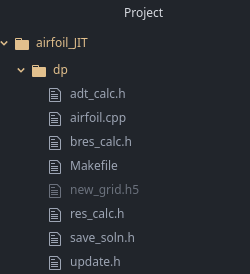
\includegraphics[width=64mm,valign=c]{files1}}
 \qquad\qquad
\subfloat[After Code Generation]{\label{fig:files_b}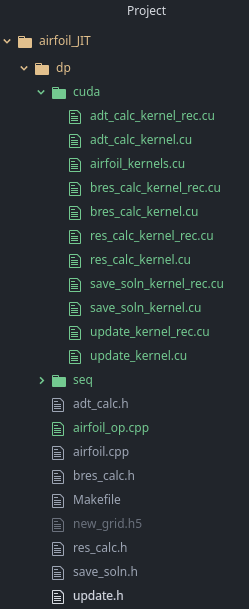
\includegraphics[width=64mm,valign=c]{files2}}
\vspace*{3in}
\end{figure}

\begin{figure}[tp]\ContinuedFloat
\centering     %%% not \center
\caption{Files in Application Folder}
\subfloat[After AOT Compile]{\label{fig:files_c}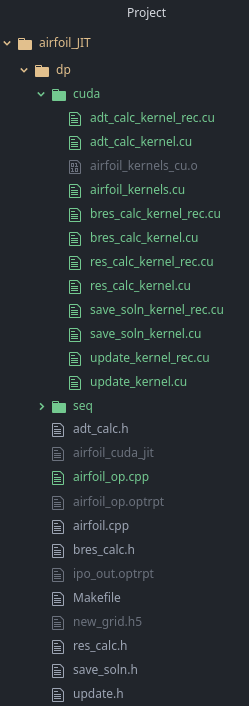
\includegraphics[width=64mm]{files3}}
 \qquad\qquad
\subfloat[After JIT Compile]{\label{fig:files_d}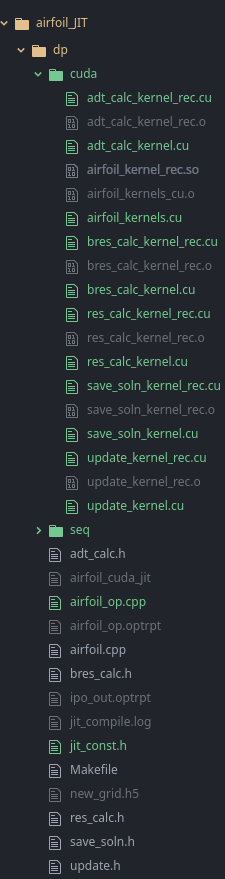
\includegraphics[width=64mm]{files4}}
\end{figure}

\subsection{Benchmarking}
Once the functionality has been confirmed to work as intended, the technique can be benchmarked to determine if there is benefit in using it for run-time efficiency. Testing was done on a personal computer with an NVIDIA GeForce MX250 Graphics Card \cite{mx250} - and while this is able to execute the CUDA code and ensure it produces the right output, it is not sufficient to gather representative benchmarking data. Using a personal computer system may result in noisy data, from the system scheduling other tasks.
\par
In order to gather better data, access to a supercomputer located in Cambridge, part of the Cambridge Service for Data-Driven Discovery (CSD3), was kindly provided - although workloads for this project were placed in a low priority queue.
\par
The supercomputer named \textit{Wilkes2} was used, which provides 4 NVidia P100 16GB Graphical Processing Units \cite{p100}. The translator currently only generates code for a single graphics card, but a possible extension would be to include MPI and divide the workload across multiple GPUs. As with many supercomputer clusters, \textit{Wilkes2} requires jobs to be submitted via SLURM \cite{slurm}.

\subsubsection{Benchmarking Strategy}
The \textit{airfoil} program is also used for benchmarking, as it is reasonably industrially representative. The input mesh remains the same as in the Testing section, with 721801 nodes, but the number of time steps is upped from 1000 to 10,000 to make any difference more noticable. OP2's internal timing funtions are used to sum the total time spent in each of the parallel loops, which can be compared between the versions with JIT compilation enabled and disabled.
\par
As seen previously in Section \ref{sss:jit_comp} (Just-in-Time Compilation), the time taken for the invocation of the compiler at runtime to complete is also recorded. It is a one-time cost at the start of execution, but still needs to be considered.
\par
Given more time other OP2 applications would also have been used to compare data, however, finding a suitable HPC system and gaining access took a larger portion of the project's duration than expected.

\subsubsection{Results}
The graph in Figure \ref{fig:res} shows the total runtime of both versions, divided sections corresponding to the total wall clock time spent in each of the parallel loops.

\begin{figure}[h!]
\begin{center}
\caption{Runtime Divided by Parallel Loop}
\label{fig:res}
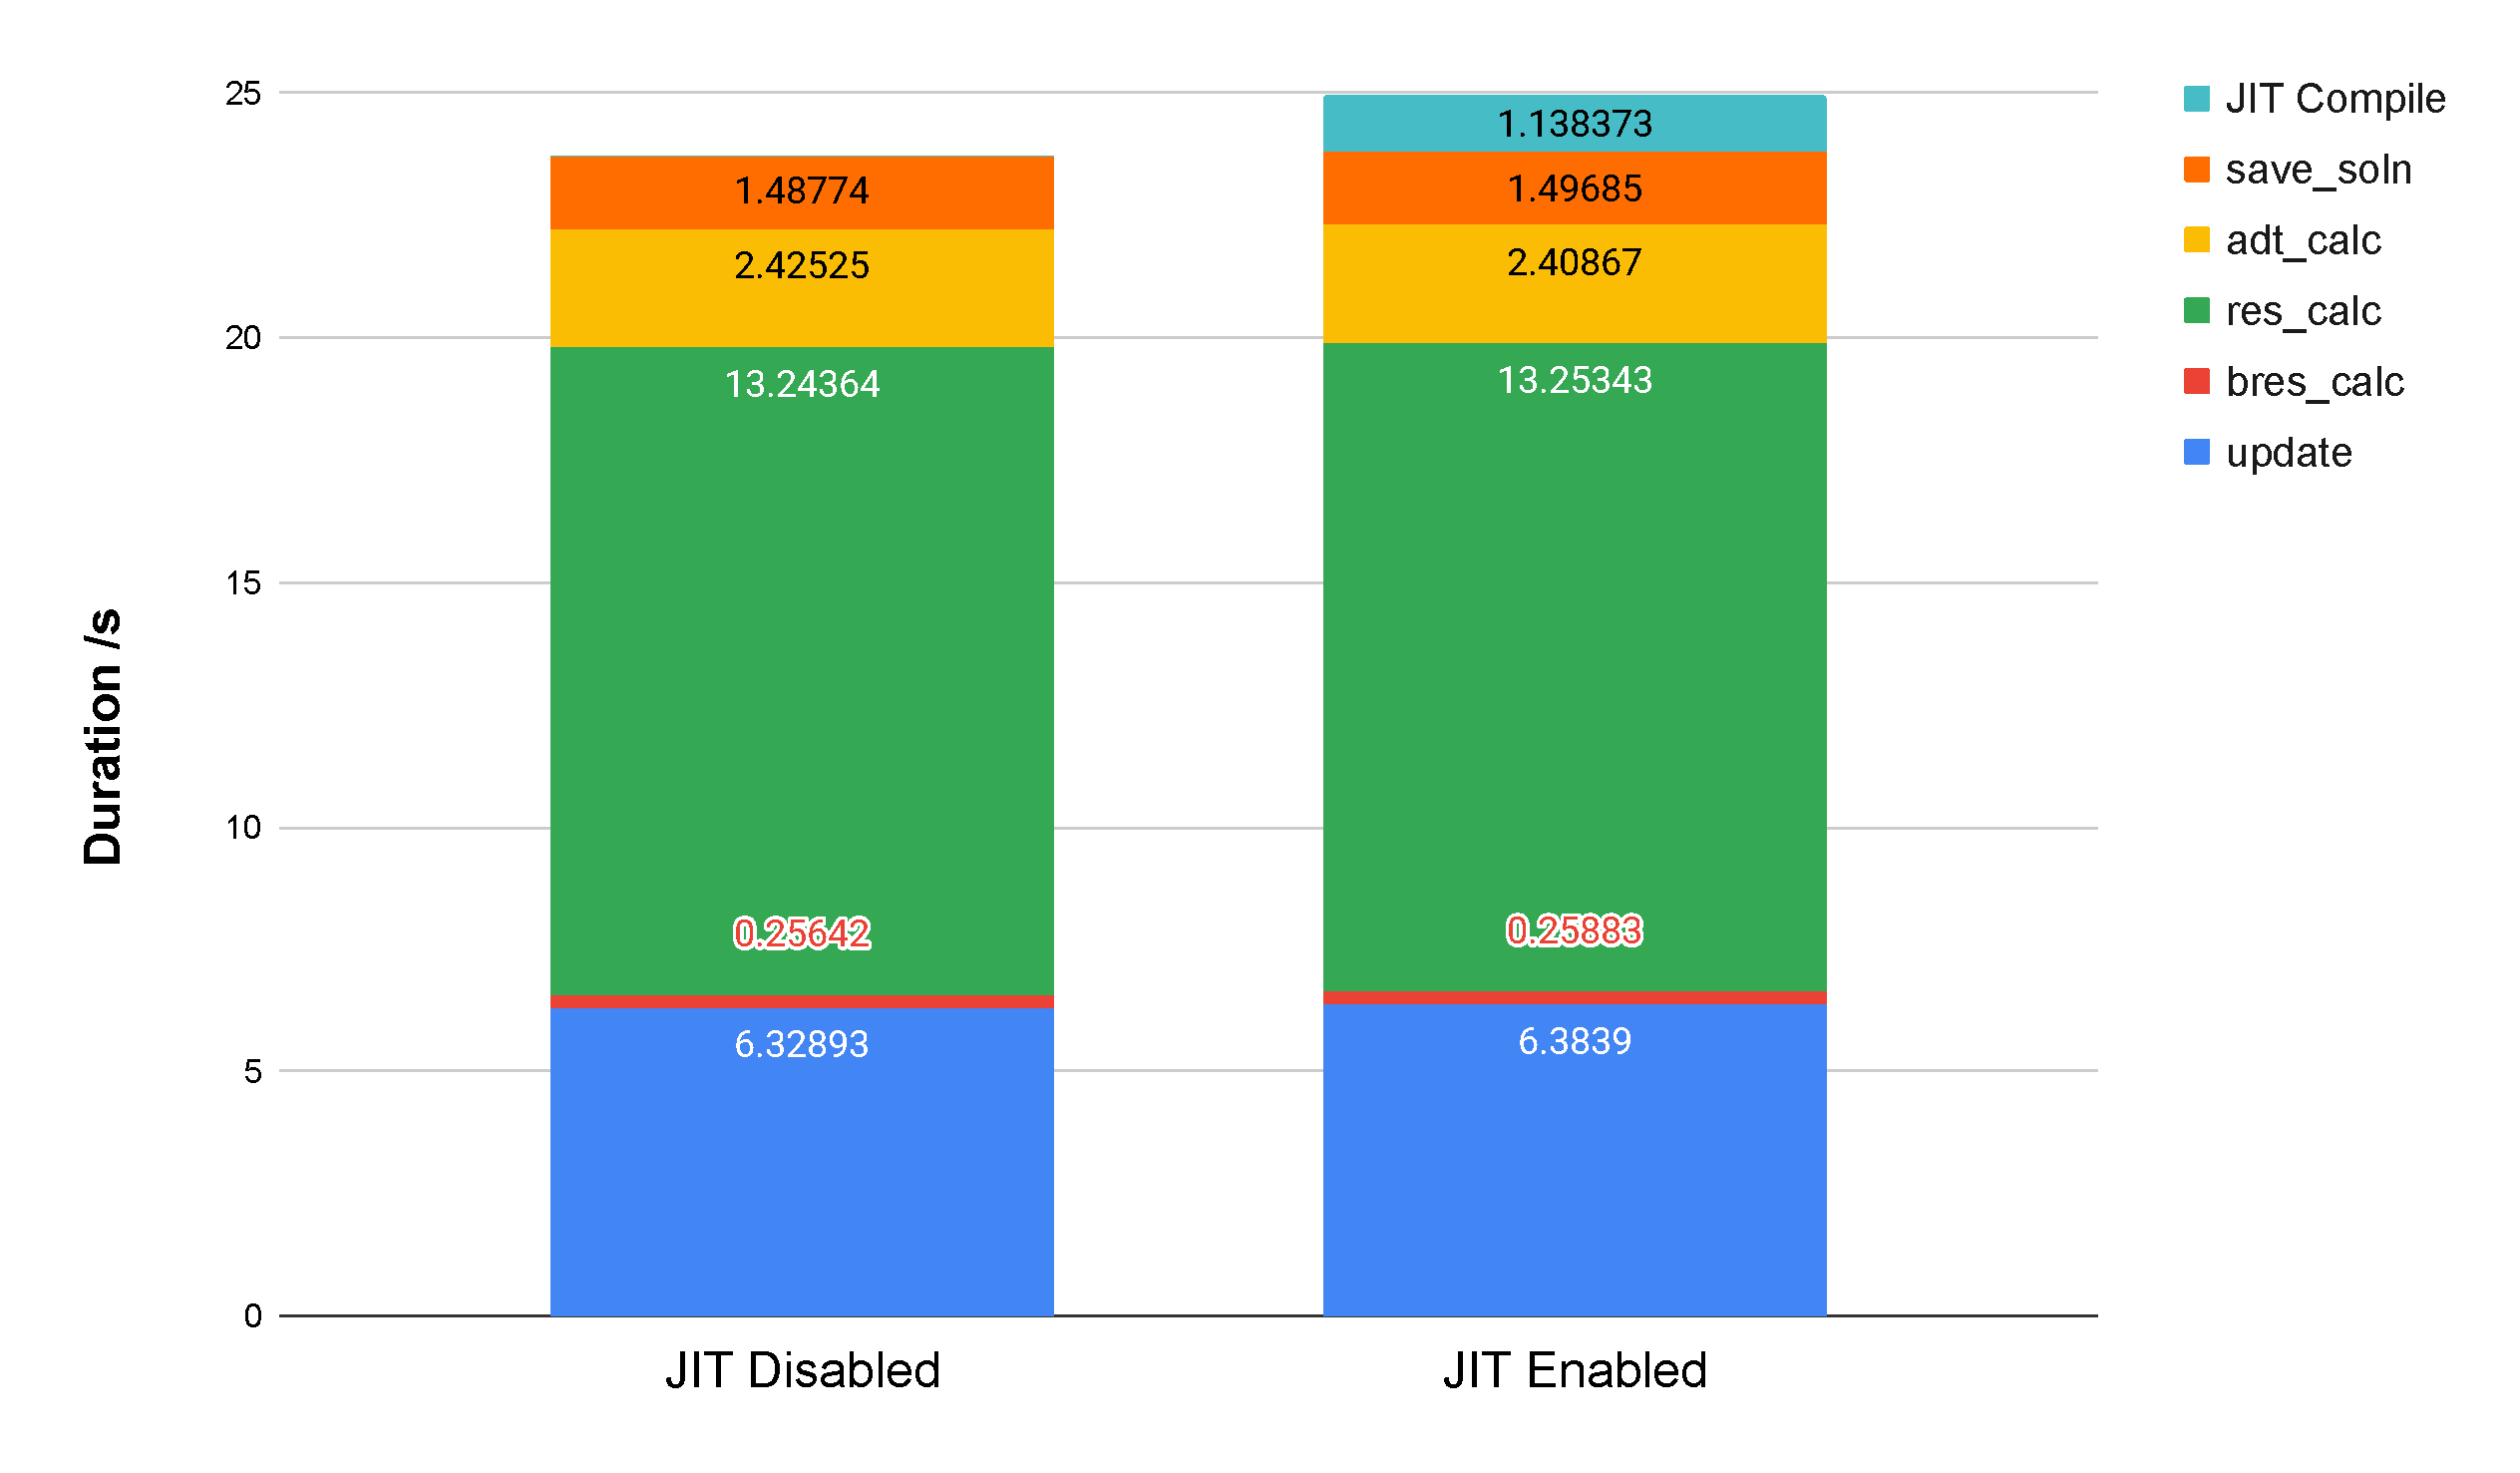
\includegraphics[width=\textwidth]{results.pdf}
\end{center}
\vspace{-1cm}
\end{figure}

\noindent Values are taken across an average of 10 executions of the binary, to further eliminate any possible noise in the JIT compilation duration.

\subsubsection{Analysis}
What Figure \ref{fig:res} clearly shows, is that the runtime has not been reduced by using the technique, and indeed is almost the same but with the addition of the time taken to invoke the compiler.
\par
It is important when drawing conclusions from this to remember that there are other assertions that can be made at runtime. Since the only assertion being made is that values declared constant will not change, the time available for optimisation is only the time taken to read constant values from memory, which will not be a significant proportion of the runtime for most projects, since CUDA-capable graphics cards have a designated section of device memory for caching constants \cite[p73]{guide}.
\par
It is true that the constants no longer need to be copied into the device memory, however this was previously only done once at the start of the program.
\par
What the results demonstrate is that more sophisticated optimisations which make use of the inputs being known need to be implemented. Since the JIT Compilation process has now been implemented, this system can continue to be used and improved upon to provide a runtime reduction to the execution of the binary. Even a small improvement to a very large solver, which might run millions of time-step iterations, could quickly re-coup and indeed begin to outweigh the relatively tiny one-time cost of recompilation.

\subsubsection{Conclusion}
Considering that this project was intended as an investigation, it can certainly be considered successful, despite not achieving the speed-up that was hoped for at the outset. Laying the groundwork for future contributors to build on top of is a worthwhile contribution to the OP2 project, and discovering that the technique of defining constants for the preprocessor is not sufficient to reduce the runtime noticably will inform future investiagations into what techniques should implemented.

